\documentclass[]{elsarticle} %review=doublespace preprint=single 5p=2 column
%%% Begin My package additions %%%%%%%%%%%%%%%%%%%
\usepackage[hyphens]{url}

  \journal{Astronomy and Computing} % Sets Journal name


\usepackage{lineno} % add

\usepackage{graphicx}
%%%%%%%%%%%%%%%% end my additions to header

\usepackage[T1]{fontenc}
\usepackage{lmodern}
\usepackage{amssymb,amsmath}
\usepackage{ifxetex,ifluatex}
\usepackage{fixltx2e} % provides \textsubscript
% use upquote if available, for straight quotes in verbatim environments
\IfFileExists{upquote.sty}{\usepackage{upquote}}{}
\ifnum 0\ifxetex 1\fi\ifluatex 1\fi=0 % if pdftex
  \usepackage[utf8]{inputenc}
\else % if luatex or xelatex
  \usepackage{fontspec}
  \ifxetex
    \usepackage{xltxtra,xunicode}
  \fi
  \defaultfontfeatures{Mapping=tex-text,Scale=MatchLowercase}
  \newcommand{\euro}{€}
\fi
% use microtype if available
\IfFileExists{microtype.sty}{\usepackage{microtype}}{}
\bibliographystyle{elsarticle-harv}
\ifxetex
  \usepackage[setpagesize=false, % page size defined by xetex
              unicode=false, % unicode breaks when used with xetex
              xetex]{hyperref}
\else
  \usepackage[unicode=true]{hyperref}
\fi
\hypersetup{breaklinks=true,
            bookmarks=true,
            pdfauthor={},
            pdftitle={Using Machine Learning to Predict the Correlation of Spectra Using SDSS Colour Magnitudes as an Improvement to the Locus Algorithm},
            colorlinks=false,
            urlcolor=blue,
            linkcolor=magenta,
            pdfborder={0 0 0}}
\urlstyle{same}  % don't use monospace font for urls

\setcounter{secnumdepth}{0}
% Pandoc toggle for numbering sections (defaults to be off)
\setcounter{secnumdepth}{0}


% tightlist command for lists without linebreak
\providecommand{\tightlist}{%
  \setlength{\itemsep}{0pt}\setlength{\parskip}{0pt}}


% Pandoc citation processing
\newlength{\cslhangindent}
\setlength{\cslhangindent}{1.5em}
\newlength{\csllabelwidth}
\setlength{\csllabelwidth}{3em}
\newlength{\cslentryspacingunit} % times entry-spacing
\setlength{\cslentryspacingunit}{\parskip}
% for Pandoc 2.8 to 2.10.1
\newenvironment{cslreferences}%
  {}%
  {\par}
% For Pandoc 2.11+
\newenvironment{CSLReferences}[2] % #1 hanging-ident, #2 entry spacing
 {% don't indent paragraphs
  \setlength{\parindent}{0pt}
  % turn on hanging indent if param 1 is 1
  \ifodd #1
  \let\oldpar\par
  \def\par{\hangindent=\cslhangindent\oldpar}
  \fi
  % set entry spacing
  \setlength{\parskip}{#2\cslentryspacingunit}
 }%
 {}
\usepackage{calc}
\newcommand{\CSLBlock}[1]{#1\hfill\break}
\newcommand{\CSLLeftMargin}[1]{\parbox[t]{\csllabelwidth}{#1}}
\newcommand{\CSLRightInline}[1]{\parbox[t]{\linewidth - \csllabelwidth}{#1}\break}
\newcommand{\CSLIndent}[1]{\hspace{\cslhangindent}#1}




\begin{document}


\begin{frontmatter}

  \title{Using Machine Learning to Predict the Correlation of Spectra
Using SDSS Colour Magnitudes as an Improvement to the Locus Algorithm}
    \author[Technological University Dublin]{Tom O'Flynn}
   \ead{tom.oflynn@tudublin.ie} 
    \author[Technological University Dublin]{Eugene Hickey\corref{1}}
   \ead{eugene.hickey@tudublin.ie} 
    \author[Technological University Dublin]{Kevin Nolan\corref{2}}
   \ead{kevin.nolan@tudublin.ie} 
    \author[Dublin Institute of Advanced Studies]{Oisin
Creaner\corref{2}}
   \ead{derek@example.com} 
      \address[Technological University Dublin]{Department of Applied
Science, Dublin D24FKT9}
    \address[Dublin Institute of Advanced Studies]{Department, Street,
City, State, Zip}
      \cortext[1]{Corresponding Author}
    \cortext[2]{Equal contribution}
  
  \begin{abstract}
  The Locus Algorithm is a new technique to improve the quality of
  differential photometry by optimising the choices of reference stars.
  At the heart of this algorithm is a routine to assess how good each
  potential reference star is by comparing its sdss magnitude values to
  those of the target star. In this way, the difference in
  wavelength-dependent effects of the Earth's atmospheric scattering
  between target and reference can be minimised. This paper sets out a
  new way to calculate the quality of each reference star using machine
  learning. A random subset of stars from sdss with spectra was chosen.
  For each one, a suitable reference star, also with a spectrum, was
  chosen. The correlation between the two spectra was taken to be the
  gold-standard measure of how well they match up for differential
  photometry. The five sdss magnitude values for each of these stars
  were used as predictors. A gradient boosting model was constructed on
  a training set of the stars and was evaluated on a testing set. The
  dataset used, the model construction, and performance evaluation are
  presented here.
  \end{abstract}
  
 \end{frontmatter}

\hypertarget{introduction}{%
\section{Introduction}\label{introduction}}

A wealth of astrophysics information is available through the study of
the brightness of celestial objects as a function of time. For example,
exoplanet detection by the transit method relies critically on
measurements of intrinsic variability where such variability can be a
small fraction of the total stellar brightness (Giltinan et al. (2011),
Everett and Howell (2001)). Ground-based observations looking for such
variability are complicated by the effects of the Earth's atmosphere
which causes incoherent wavelength-dependent variations in the stellar
flux detected. This can mask intrinsic variability and hamper the study
of variable astrophysical phenomena (Smith et al. (2008)).

The technique of differential photometry has been developed in an
attempt to mitigate the effects of the Earth's atmosphere on studies of
stellar variability. Differential photometry uses references stars at
small angular separations from the star of interest as comparators.
Atmospheric effects should have similar effects on the measured flux
from all of these stars causing them to vary in unison (Burdanov et al.
(2014)). Because scattering in the Earth's atmosphere is wavelength
dependent, the technique is especially successful if the target star and
reference stars are spectrally similar (Milone and Pel (2011), Sterken
et al. (2011)).

The Locus Algorithm (Creaner et al. (2022)) has been used to create
catalogues of pointings suitable for differential photometry on
astromonical targets based on a novel technique of choosing appropriate
reference stars (Creaner et al. (2020) and Creaner EXO's). The algorithm
no longer places the target in the centre of the field of view but in
general, repositions it so as to include the best set of reference
stars. Assessment of each reference star is performed by referring to
the sdss catalogue and the colour band magnitudes therein. These
magnitudes can be used to infer the overall shape of the star's
spectrum. Stars that have similar spectra with be effected by scattering
from the Earth's atmosphere to a more comparable degree that stars with
dissimilar spectra. The original Locus Algorithm used a rational, but
ad-hoc, method to estimate the correlation of stellar spectra based on
differences between their g, r, and i sdss colour magnitudes (Creaner
{[}Thesis{]} (2017)). This was necessary for computational efficiency.
The work presented here presents a more rigorous technique to estimate
the correlation of stellar spectra based on machine learning. The subset
of stars in sdss that have their spectra measured are used. These stars
are paired off such that each pair has similar colour magnitude
differences and are thus potentially a good match for differential
photometry. This corresponds to the pre-filtering step employed by
Creaner {[}Thesis{]} (2017). The correlation between each pairs spectra
is calculated. This forms the basis of a goodness-of-fit between the two
spectra. The sdss magnitudes (u, g, r, i, and z for both stars in the
pair) are then used to train a machine learning algorithm to predict
this goodness-of-fit. The model produced is then applied to other pairs
of stars, the test set, to evaluate its performance. The results show a
significant improvement over the original ad-hoc Locus Algorithm
routine, this model will be incorporated to future generations of the
Locus Algorithm.

\hypertarget{data}{%
\section{Data}\label{data}}

This work uses 5591 stellar spectra from the SDSS SEGUE and BOSS
observations and their physical parameters from the 13th SDSS data
release (Aguado et al. (2018)). The spectra are clipped to just the
wavelengths contained in the sdss r band (between 550nm and 700nm).
Stars are paired off based on their sdss colour magnitudes so that both
stars in a pair are of similar colour. Specifically, both
\((g_1-r_1)-(g_2-r_2)\) and \((r_1-i_1)-(r_2-i_2)\) will be between 0
and 0.1. This ensures that these stars would be realistic matches for
differential photometry. In addition, stars were chosen that had r
colour magnitude values between 15 and 20. The SQL queries used to
download physical parameters and the spectra are given in the
supplementary materials for this paper. Correlations between spectra are
calculated using the usual Pearson Correlation formula, equation
(\ref{eq:correlation}).

\begin{equation}
  \displaystyle r_{xy}={\frac {n\sum x_{i}y_{i}-\sum x_{i}\sum y_{i}}{{\sqrt {n\sum x_{i}^{2}-\left(\sum x_{i}\right)^{2}}}~{\sqrt {n\sum y_{i}^{2}-\left(\sum y_{i}\right)^{2}}}}}.
  \label{eq:correlation}
\end{equation}

where \(x_i\) refer to the flux from the first star at a given
wavelength, \(i\), in units of \(erg/cm^2/s Å\), \(y_i\) the flux from
the second star at the same wavelength. Figure \ref{fig:spectra} shows
some pairs of stars along with their correlations. The first pair, A and
B, are representative of the sample. The second pair, C and D, were
chosen to have an unusually low correlation for this sample set.

\begin{figure}
  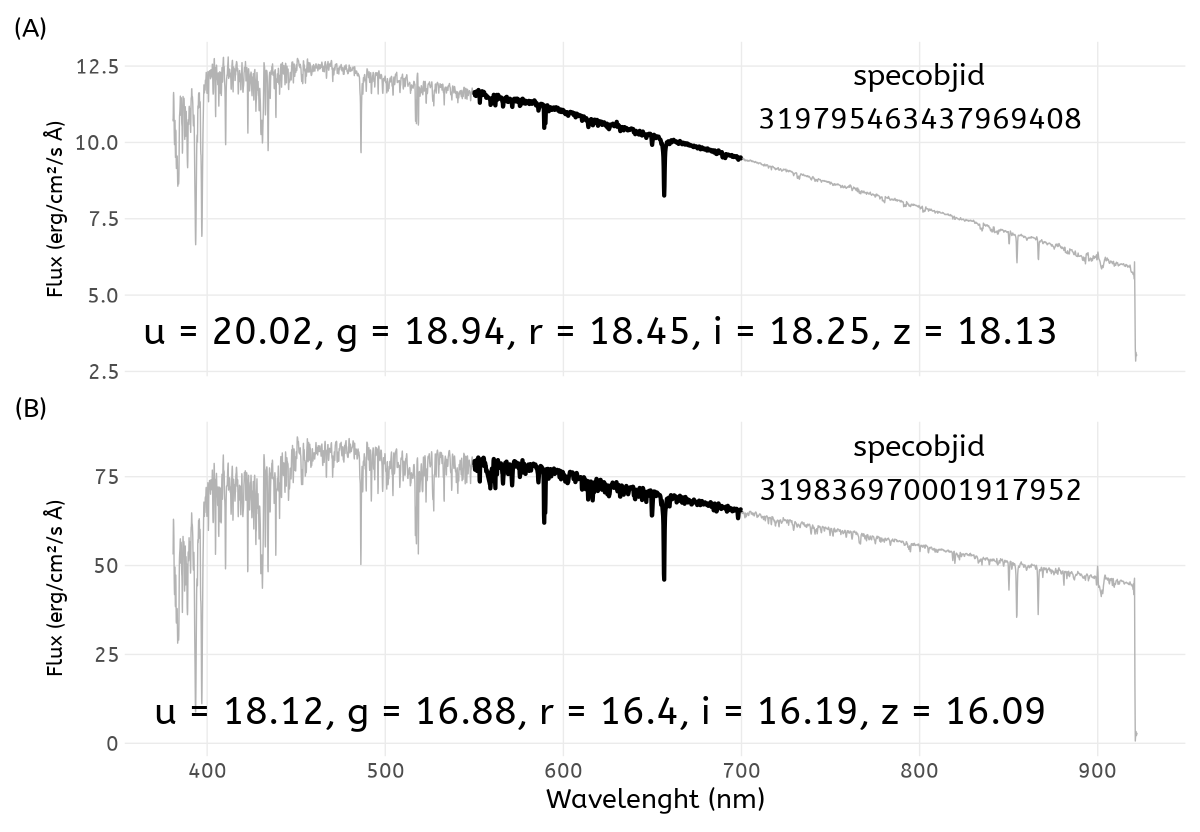
\includegraphics[width=\columnwidth, height = 8cm]{figures/spectra1}
  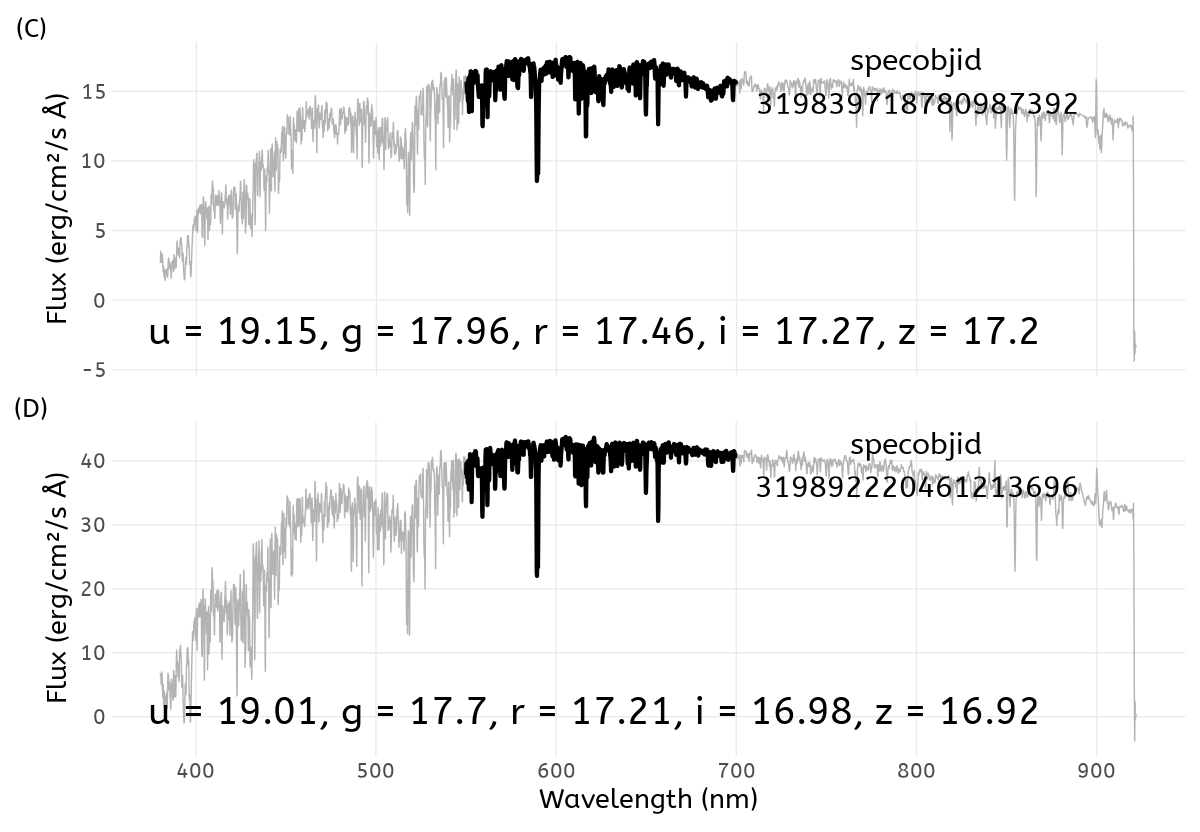
\includegraphics[width=\columnwidth, height = 8cm]{figures/spectra2}
    \caption{Two pairs of spectra downloaded from SDSS. The ugriz colour magnitudes for each star is given below its spectrum. The darkened area of the spectral line corresponds to the r-band wavelengths. The correlation between spectra A and C is 0.96. That between spectra B and D is 0.75.}
    \label{fig:spectra}
\end{figure}

Correlation is usually bounded by -1 and 1. And because these are
spectra from stars and they have similar colour magnitudes, the
correlations tend to be clustered near this higher end, see the
histogram in figure \ref{fig:histograms}A below. Machine learning
algorithms work better with normally distributed values (need reference)
and this is especially true when it comes to analysing model performance
(another reference), so the correlation values were transformed. First
of all by a logit transformation (\ref{eq:logit}):

\begin{equation}
  \displaystyle \operatorname {logit} (x)=\ln \left({\frac {1+x}{1-x}}\right)
  \label{eq:logit}
\end{equation}

And then by scaling and normalising the values to have a mean of 0 and a
standard deviation of 1. The resulting transformed values are shown in
figure \ref{fig:histograms}B.

\begin{figure}
  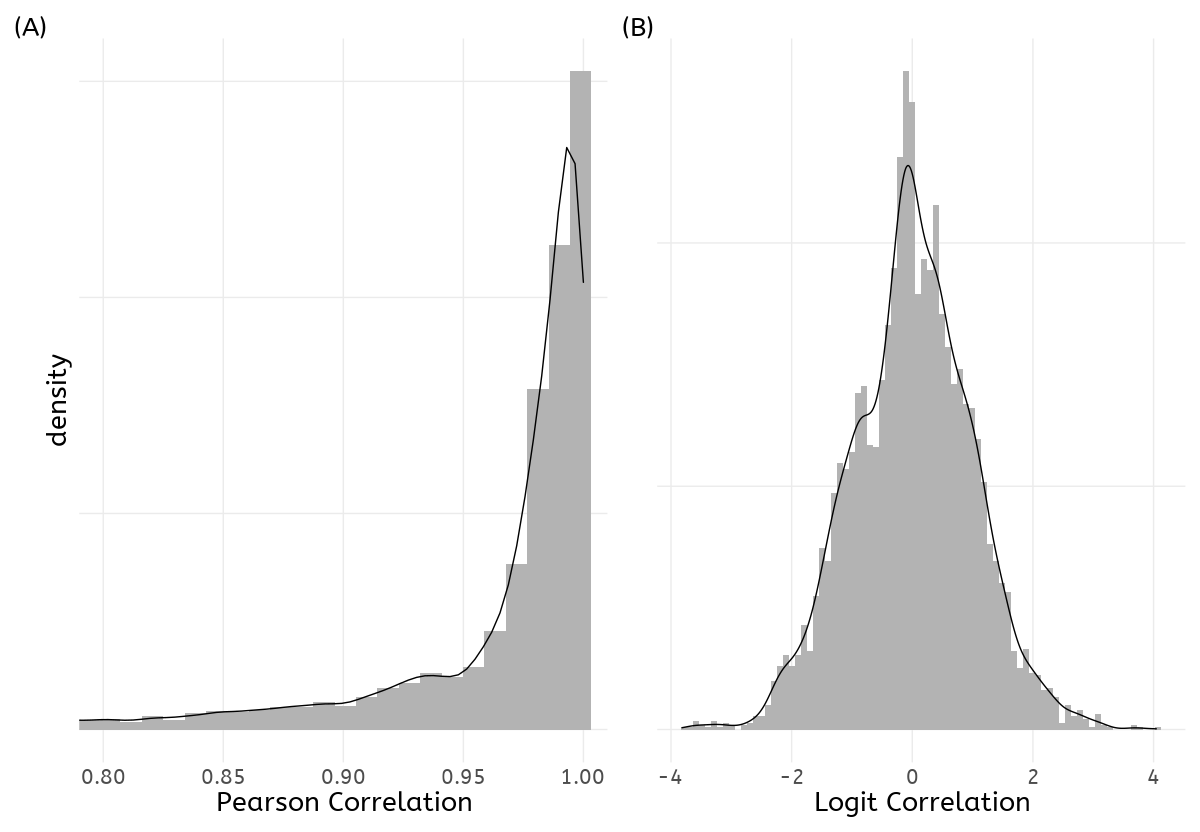
\includegraphics[width=\columnwidth, height = 5cm]{figures/histograms}
    \caption{(A) Histogram of Pearson correlation values between r-band spectra between pairs of matched stars. (B) Values in (A) transformed by a logit function.}
    \label{fig:histograms}
\end{figure}

The data is split into test and training sets, with 70\% of the data
(3915 samples) in the training set and the remainder in the test set.
Each set has a representative sample of correlation values, to do this
the original sample of 5591 pairs is split into five groups based on
percentiles of the correlation and both testing and training sets get a
commensurate proportion of each group.

\hypertarget{model}{%
\section{Model}\label{model}}

A regression model was built on the training set, using the ugriz values
for both stars in each pair as predictors for the logit(correlation)
value. An eXtreme Gradient Boosting model (Friedman et al. (2000), Chen
and Guestrin (2021)) was used. This was chosen because of its
performance and reliability (Bentéjac et al. (2020)). Cross validation
was performed using a bootstrap method (Efron (1983)). The model was fit
with the maximum number of boosting iterations set to 150, the learning
rate set to 0.3, the maximum tree depth set to 3. It was set to minimise
the RMSE on the training set. The final model fit was produced after 106
iterations.

One of the 150 trees produced is shown in figure \ref{fig:tree}.

\begin{figure}
  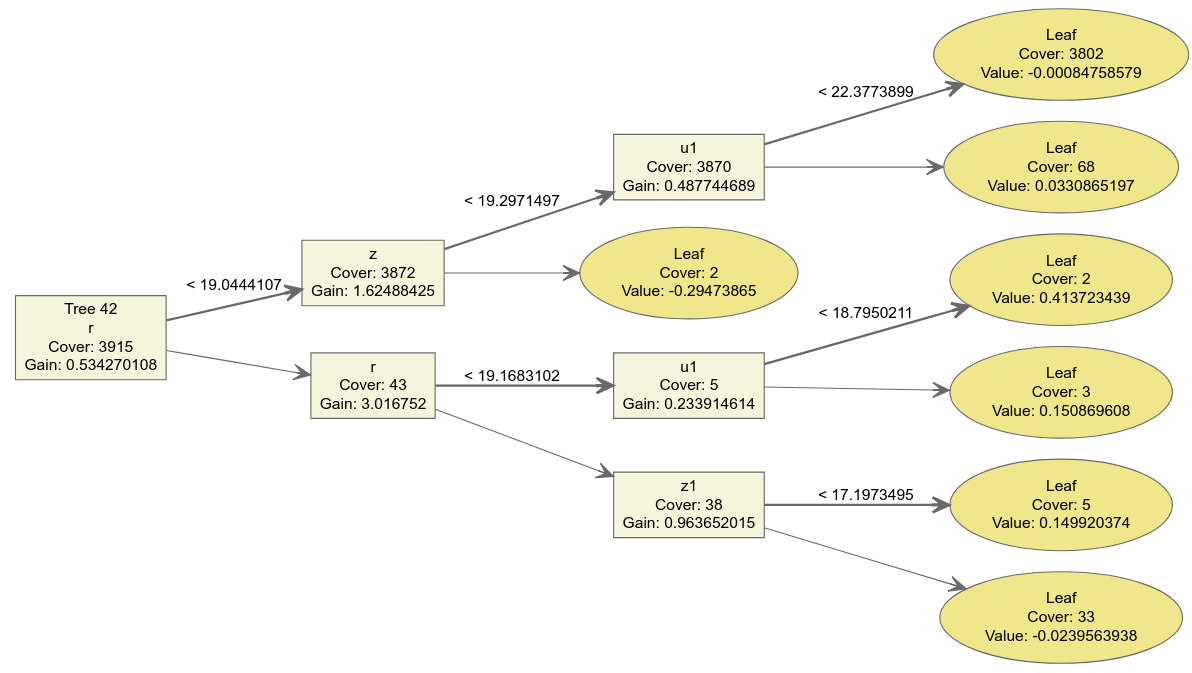
\includegraphics[width=\columnwidth, height = 6.5cm]{figures/tree}
    \caption{One of the 150 decision trees produced by the gradient boosting algorithm}
    \label{fig:tree}
\end{figure}

\hypertarget{model-evaluation}{%
\section{Model Evaluation}\label{model-evaluation}}

The model was then used to predict the logit correlation values from the
1676 star pairs from the test set. Figure \ref{fig:obs-pred} shows the
resulting values of observed logit correlation values against predicted
logit correlation values. Figure \ref{fig:residuals-pred} shows the
resulting values of the residuals, the observations minus the predicted
values, against predicted logit correlation values. Figure
\ref{fig:residuals-hist} shows a histogram of the residual values,
figure \ref{fig:residuals-qq} shows a quantile-quantile (QQ) plot of the
residuals. The shape of this last plot shows the residuals to be
somewhat platykurtic which is acceptable for a machine learning fit
(ref???).

The \(R^2\) value of predicted logit correlation on the test set was
found to be 71\%. The RMSE on the test set was found to be 0.55. The
performance of the original function used in Creaner et al. (2022) was
worse, with an \(R^2\) of 13\%.

\begin{figure}
  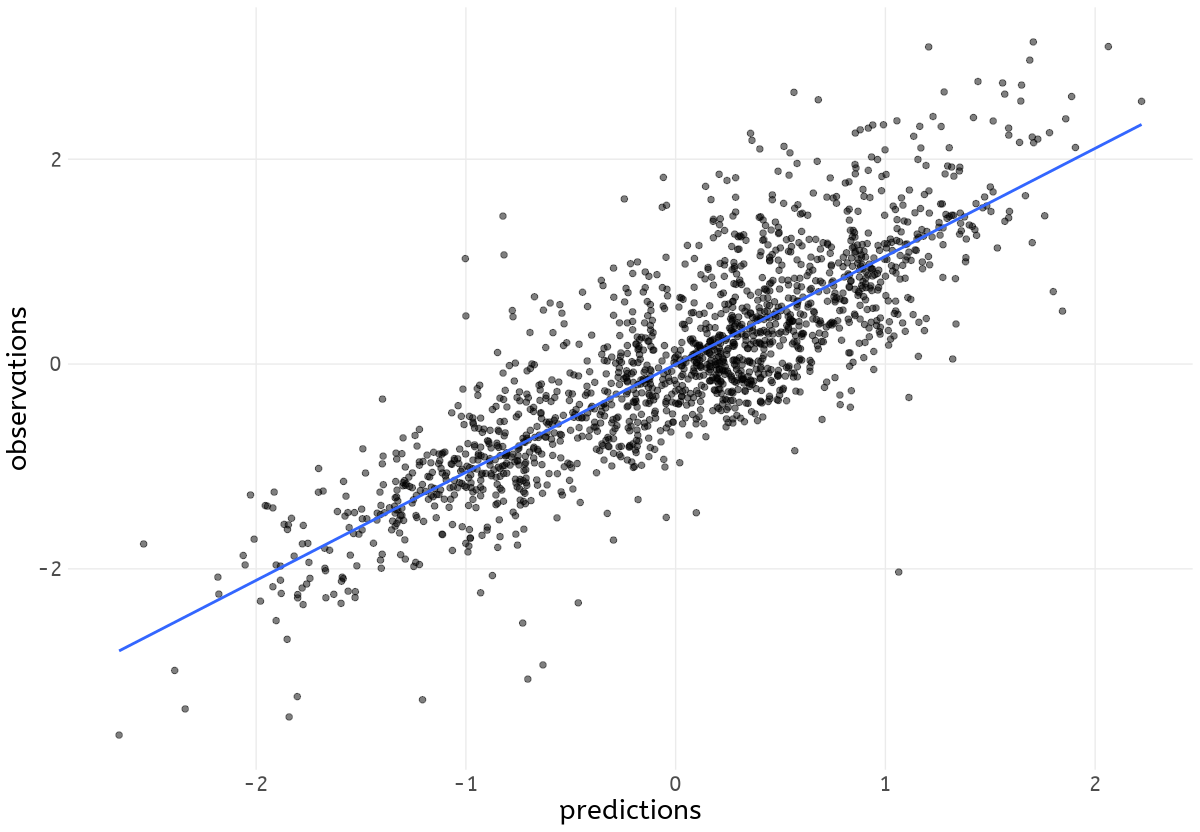
\includegraphics[width=\columnwidth, height = 6.5cm]{figures/observed-predicted}
    \caption{Observed versus predicted logit correlation values}
    \label{fig:obs-pred}
\end{figure}

\begin{figure}
  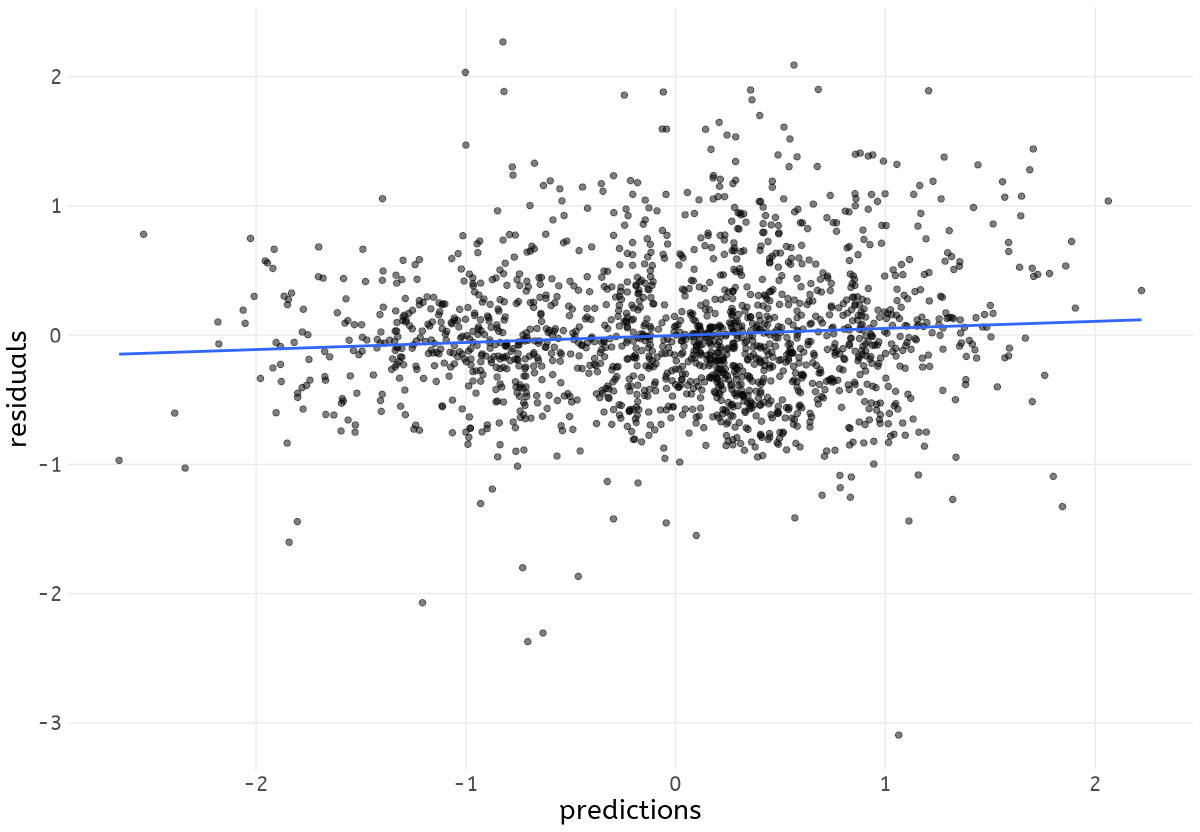
\includegraphics[width=\columnwidth, height = 6.5cm]{figures/residuals-predicted}
    \caption{Residuals versus predicted logit correlation values}
    \label{fig:residuals-pred}
\end{figure}

\begin{figure}
  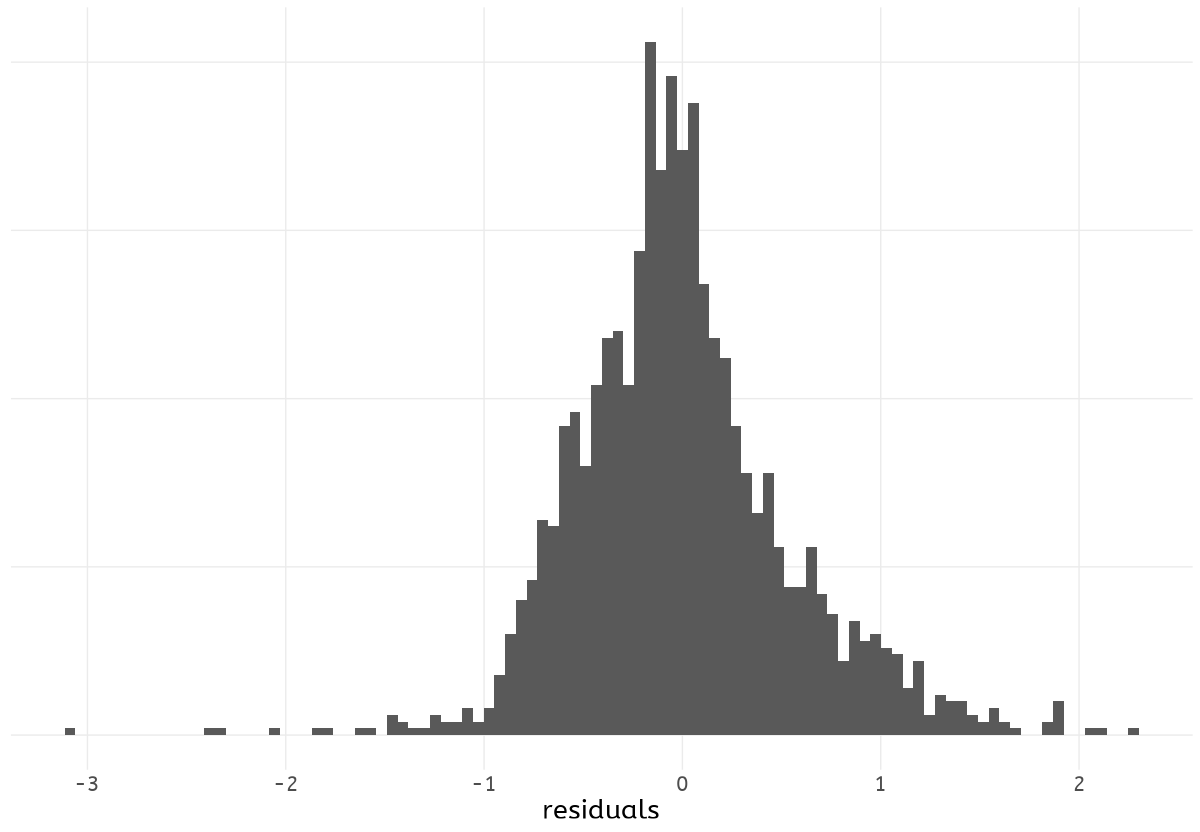
\includegraphics[width=\columnwidth, height = 6.5cm]{figures/residuals-hist}
    \caption{Observed versus predicted logit correlation values}
    \label{fig:residuals-hist}
\end{figure}

\begin{figure}
  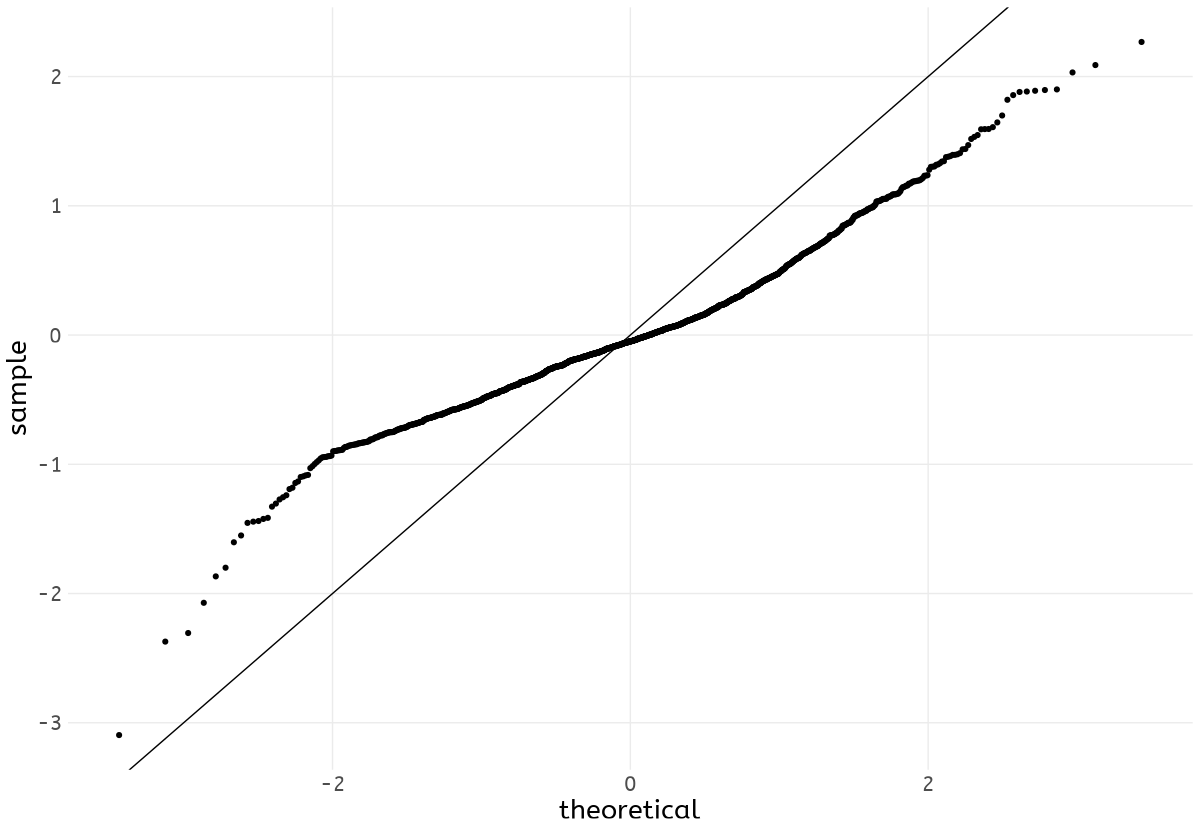
\includegraphics[width=\columnwidth, height = 6.5cm]{figures/residuals-qq}
    \caption{Observed versus predicted logit correlation values}
    \label{fig:residuals-qq}
\end{figure}

\hypertarget{conclusions}{%
\section{Conclusions}\label{conclusions}}

The last numbered section should briefly summarise what has been done,
and describe the final conclusions which the authors draw from their
work.

\hypertarget{references}{%
\section*{References}\label{references}}
\addcontentsline{toc}{section}{References}

\hypertarget{refs}{}
\begin{CSLReferences}{1}{0}
\leavevmode\vadjust pre{\hypertarget{ref-Aguado2018}{}}%
Aguado, D.S., Ahumada, R., Almeida, A., Anderson, S.F., Andrews, B.H.,
Anguiano, B., Ortiz, E.A., Aragon-Salamanca, A., Argudo-Fernandez, M.,
Aubert, M., Avila-Reese, V., Badenes, C., Rembold, S.B., Barger, K.,
Barrera-Ballesteros, J., Bates, D., Bautista, J., Beaton, R.L., Beers,
T.C., Belfiore, F., Bernardi, M., Bershady, M., Beutler, F., Bird, J.,
Bizyaev, D., Blanc, G.A., Blanton, M.R., Blomqvist, M., Bolton, A.S.,
Boquien, M., Borissova, J., Bovy, J., Brandt, W.N., Brinkmann, J.,
Brownstein, J.R., Bundy, K., Burgasser, A., Byler, N., Diaz, M.C.,
Cappellari, M., Carrera, R., Sodi, B.C., Chen, Y., Cherinka, B., Choi,
P.D., Chung, H., Coffey, D., Comerford, J.M., Comparat, J., Covey, K.,
Ilha, G. da S., Costa, L. da, Dai, Y.S., Damke, G., Darling, J., Davies,
R., Dawson, K., Agathe, V. de S., Machado, A.D., Del Moro, A., De Lee,
N., Diamond-Stanic, A.M., Sanchez, H.D., Donor, J., Drory, N., Bourboux,
H. du M. des, Duckworth, C., Dwelly, T., Ebelke, G., Emsellem, E.,
Escoffier, S., Fernandez-Trincado, J.G., Feuillet, D., Fischer, J.-L.,
Fleming, S.W., Fraser-McKelvie, A., Freischlad, G., Frinchaboy, P.M.,
Fu, H., Galbany, L., Garcia-Dias, R., Garcia-Hernandez, D.A., Oehmichen,
L.A.G., Maia, M.A.G., Gil-Marin, H., Grabowski, K., Gu, M., Guo, H., Ha,
J., Harrington, E., Hasselquist, S., Hayes, C.R., Hearty, F., Toledo,
H.H., Hicks, H., Hogg, D.W., Holley-Bockelmann, K., Holtzman, J.A.,
Hsieh, B.-C., Hunt, J.A.S., Hwang, H.S., Ibarra-Medel, H.J., Angel,
C.E.J., Johnson, J., Jones, A., Jonsson, H., Kinemuchi, K., Kollmeier,
J., Krawczyk, C., Kreckel, K., Kruk, S., Lacerna, I., Lan, T.-W., Lane,
R.R., Law, D.R., Lee, Y.-B., Li, C., Lian, J., Lin, L., Lin, Y.-T.,
Lintott, C., Long, D., Longa-Pena, P., Mackereth, J.T., Macorra, A. de
la, Majewski, S.R., Malanushenko, O., Manchado, A., Maraston, C.,
Mariappan, V., Marinelli, M., Marques-Chaves, R., Masseron, T., Masters,
K.L., McDermid, R.M., Pena, N.M., Meneses-Goytia, S., Merloni, A.,
Merrifield, M., Meszaros, S., Minniti, D., Minsley, R., Muna, D., Myers,
A.D., Nair, P., Nascimento, J.C. do, Newman, J.A., Nitschelm, C.,
Olmstead, M.D., Oravetz, A., Oravetz, D., Minakata, R.A.O., Pace, Z.,
Padilla, N., Palicio, P.A., Pan, K., Pan, H.-A., Parikh, T., Parker, J.,
Peirani, S., Penny, S., Percival, W.J., Perez-Fournon, I., Peterken, T.,
Pinsonneault, M., Prakash, A., Raddick, J., Raichoor, A., Riffel, R.A.,
Riffel, R., Rix, H.-W., Robin, A.C., Roman-Lopes, A., Rose, B., Ross,
A.J., Rossi, G., Rowlands, K., Rubin, K.H.R., Sanchez, S.F.,
Sanchez-Gallego, J.R., Sayres, C., Schaefer, A., Schiavon, R.P.,
Schimoia, J.S., Schlafly, E., Schlegel, D., Schneider, D., Schultheis,
M., Seo, H.-J., Shamsi, S.J., Shao, Z., Shen, S., Shetty, S., Simonian,
G., Smethurst, R., Sobeck, J., Souter, B.J., Spindler, A., Stark, D.V.,
Stassun, K.G., Steinmetz, M., Storchi-Bergmann, T., Stringfellow, G.S.,
Suarez, G., Sun, J., Taghizadeh-Popp, M., Talbot, M.S., Tayar, J.,
Thakar, A.R., Thomas, D., Tissera, P., Tojeiro, R., Troup, N.W.,
Unda-Sanzana, E., Valenzuela, O., Na, M.V.-M., Mata, J.A.V., Wake, D.,
Weaver, B.A., Weijmans, A.-M., Westfall, K.B., Wild, V., Wilson, J.,
Woods, E., Yan, R., Yang, M., Zamora, O., Zasowski, G., Zhang, K.,
Zheng, Z., Zheng, Z., Zhu, G., Zinn, J.C., Zou, H., 2018. {The Fifteenth
Data Release of the Sloan Digital Sky Surveys: First Release of MaNGA
Derived Quantities, Data Visualization Tools and Stellar Library}.
doi:\href{https://doi.org/10.3847/1538-4365/aaf651}{10.3847/1538-4365/aaf651}

\leavevmode\vadjust pre{\hypertarget{ref-Bentejac2020}{}}%
Bentéjac, C., Csörgő, A., Martínez-Muñoz, G., 2020. {A comparative
analysis of gradient boosting algorithms}. Artificial Intelligence
Review 2020 54:3 54, 1937--1967.
doi:\href{https://doi.org/10.1007/S10462-020-09896-5}{10.1007/S10462-020-09896-5}

\leavevmode\vadjust pre{\hypertarget{ref-Burdanov2014}{}}%
Burdanov, A.Y., Krushinsky, V.V., Popov, A.A., 2014. {Astrokit-an
Efficient Program for High-Precision Differential CCD Photometry and
Search for Variable Stars}. Translated from Astrofizicheskij Byulleten
69.

\leavevmode\vadjust pre{\hypertarget{ref-Chen2021}{}}%
Chen, T., Guestrin, C., 2021. {Extreme Gradient Boosting {[}R package
xgboost version 1.5.0.2{]}}. Proceedings of the ACM SIGKDD International
Conference on Knowledge Discovery and Data Mining 13-17-Augu, 785--794.
doi:\href{https://doi.org/10.1145/2939672.2939785}{10.1145/2939672.2939785}

\leavevmode\vadjust pre{\hypertarget{ref-creaner2022}{}}%
Creaner, O., Nolan, K., Hickey, E., Smith, N., 2022. {The Locus
Algorithm: A novel technique for identifying optimised pointings for
differential photometry}. Astronomy and Computing 38, 100537.
doi:\href{https://doi.org/10.1016/J.ASCOM.2021.100537}{10.1016/J.ASCOM.2021.100537}

\leavevmode\vadjust pre{\hypertarget{ref-creaner2020}{}}%
Creaner, O., Nolan, K., Smith, N., Grennan, D., Hickey, E., 2020. {A
catalogue of Locus Algorithm pointings for optimal differential
photometry for 23 779 quasars}. Monthly Notices of the Royal
Astronomical Society 498, 3720--3729.
doi:\href{https://doi.org/10.1093/MNRAS/STAA2494}{10.1093/MNRAS/STAA2494}

\leavevmode\vadjust pre{\hypertarget{ref-Creaner2017}{}}%
Creaner {[}Thesis{]}, O., 2017. {Data Mining by Grid Computing in the
Search for Extrasolar Planets}. Doctoral.
doi:\url{https://doi.org/10.21427/7w45-6018}

\leavevmode\vadjust pre{\hypertarget{ref-Efron1983}{}}%
Efron, B., 1983. {Estimating the error rate of a prediction rule:
Improvement on cross-validation}. Journal of the American Statistical
Association 78, 316--331.
doi:\href{https://doi.org/10.1080/01621459.1983.10477973}{10.1080/01621459.1983.10477973}

\leavevmode\vadjust pre{\hypertarget{ref-Everett2001}{}}%
Everett, M.E., Howell, S.B., 2001. {A Technique for Ultrahigh‐Precision
CCD Photometry}. Publications of the Astronomical Society of the Pacific
113, 1428--1435.
doi:\href{https://doi.org/10.1086/323387/0}{10.1086/323387/0}

\leavevmode\vadjust pre{\hypertarget{ref-Friedman2000}{}}%
Friedman, J., Hastie, T., Tibshirani, R., 2000. {Additive logistic
regression: A statistical view of boosting}. Annals of Statistics 28,
337--407.
doi:\href{https://doi.org/10.1214/AOS/1016218223}{10.1214/AOS/1016218223}

\leavevmode\vadjust pre{\hypertarget{ref-Giltinan2011}{}}%
Giltinan, A., Loughnan, D., Collins, A., Smith, N., 2011. {Using EMCCD's
to improve the photometric precision of ground-based astronomical
observations}. Journal of Physics: Conference Series 307.
doi:\href{https://doi.org/10.1088/1742-6596/307/1/012010}{10.1088/1742-6596/307/1/012010}

\leavevmode\vadjust pre{\hypertarget{ref-Milone2011a}{}}%
Milone, E.F., Pel, J.W., 2011. {The High Road to Astronomical
Photometric Precision: Differential Photometry} 33--68.
doi:\href{https://doi.org/10.1007/978-1-4419-8050-2_2}{10.1007/978-1-4419-8050-2\_2}

\leavevmode\vadjust pre{\hypertarget{ref-Smith2008}{}}%
Smith, N., Giltinan, A., O'Connor, A., O'Driscoll, S., Collins, A.,
Loughnan, D., Papageorgiou, A., Smith, N., Giltinan, A., O'Connor, A.,
O'Driscoll, S., Collins, A., Loughnan, D., Papageorgiou, A., 2008.
{EMCCD Technology in High Precision Photometry on Short Timescales}.
ASSL 351, 257.
doi:\href{https://doi.org/10.1007/978-1-4020-6518-7_13}{10.1007/978-1-4020-6518-7\_13}

\leavevmode\vadjust pre{\hypertarget{ref-Sterken2011}{}}%
Sterken, C., Milone, E.F., Young, A.T., 2011. {Photometric Precision and
Accuracy} 1--32.
doi:\href{https://doi.org/10.1007/978-1-4419-8050-2_1}{10.1007/978-1-4419-8050-2\_1}

\end{CSLReferences}

\appendix

\hypertarget{some-extra-material}{%
\section{Some extra material}\label{some-extra-material}}

If you want to present additional material which would interrupt the
flow of the main paper, it can be placed in an Appendix which appears
after the list of references.


\end{document}
